%% Copernicus Publications Manuscript Preparation Template for LaTeX Submissions
%% ---------------------------------
%% This template should be used for copernicus.cls
%% The class file and some style files are bundled in the Copernicus Latex Package which can be downloaded from the different journal webpages.
%% For further assistance please contact the Copernicus Publications at: publications@copernicus.org
%% http://publications.copernicus.org


%% Please use the following documentclass and Journal Abbreviations for Discussion Papers and Final Revised Papers.


%% 2-Column Papers and Discussion Papers
\documentclass[esd, manuscript]{copernicus}



%% Journal Abbreviations (Please use the same for Discussion Papers and Final Revised Papers)

% Archives Animal Breeding (aab)
% Atmospheric Chemistry and Physics (acp)
% Advances in Geosciences (adgeo)
% Advances in Statistical Climatology, Meteorology and Oceanography (ascmo)
% Annales Geophysicae (angeo)
% ASTRA Proceedings (ap)
% Atmospheric Measurement Techniques (amt)
% Advances in Radio Science (ars)
% Advances in Science and Research (asr)
% Biogeosciences (bg)
% Climate of the Past (cp)
% Drinking Water Engineering and Science (dwes)
% Earth System Dynamics (esd)
% Earth Surface Dynamics (esurf)
% Earth System Science Data (essd)
% Fossil Record (fr)
% Geographica Helvetica (gh)
% Geoscientific Instrumentation, Methods and Data Systems (gi)
% Geoscientific Model Development (gmd)
% Geothermal Energy Science (gtes)
% Hydrology and Earth System Sciences (hess)
% History of Geo- and Space Sciences (hgss)
% Journal of Sensors and Sensor Systems (jsss)
% Mechanical Sciences (ms)
% Natural Hazards and Earth System Sciences (nhess)
% Nonlinear Processes in Geophysics (npg)
% Ocean Science (os)
% Proceedings of the International Association of Hydrological Sciences (piahs)
% Primate Biology (pb)
% Scientific Drilling (sd)
% SOIL (soil)
% Solid Earth (se)
% The Cryosphere (tc)
% Web Ecology (we)
% Wind Energy Science (wes)


%% \usepackage commands included in the copernicus.cls:
%\usepackage[german, english]{babel}
%\usepackage{tabularx}
%\usepackage{cancel}
%\usepackage{multirow}
%\usepackage{supertabular}
%\usepackage{algorithmic}
%\usepackage{algorithm}
%\usepackage{amsthm}
%\usepackage{float}
%\usepackage{subfig}
%\usepackage{rotating}


\begin{document}

\title{TEXT}


% \Author[affil]{given_name}{surname}

\Author[1]{Doug}{McNeall}
\Author[2]{Jonny}{Williams}
\Author[1]{Ben}{Booth}
\Author[1]{Richard}{Betts}
\Author[3]{Peter}{Challenor}
\Author[1]{Andrew}{Wiltshire}
\Author[1]{David}{Sexton}


\affil[1]{Met Office Hadley Centre, FitzRoy Road, Exeter, EX1 3PB UK}
\affil[2]{NIWA, New Zealand}
\affil[3]{University of Exeter, North Park Road, Exeter EX4 4QE UK}

%% The [] brackets identify the author with the corresponding affiliation. 1, 2, 3, etc. should be inserted.



\runningtitle{TEXT}

\runningauthor{TEXT}

\correspondence{Doug McNeall (doug.mcneall@metoffice.gov.uk)}



\received{}
\pubdiscuss{} %% only important for two-stage journals
\revised{}
\accepted{}
\published{}

%% These dates will be inserted by Copernicus Publications during the typesetting process.


\firstpage{1}

\maketitle



\begin{abstract}
We use observations of forest fraction to constrain carbon cycle and land surface input parameters of the reduced resolution global climate model, FAMOUS. Using a history matching approach along with a computationally cheap statistical proxy (emulator) of the climate model, we compare an ensemble of simulations of forest fraction with observations, and rule out parameter settings where the forests are poorly simulated. 

Regions of parameter space where FAMOUS best simulates the Amazon forest fraction are incompatible with the regions where FAMOUS best simulates other forests. Previous studies using climate models have used similar methods to find previously untried candidate input parameter sets that remove what was assumed an underlying structural error. We offer a counter example, arguing that we have found a true structural discrepancy. This has implications for the calibration of FAMOUS: using observations of different forest regions to calibrate the model leads to very different conclusions about the best values, the corresponding uncertainty of input parameters, and potentially, predictions of future forest cover. Dealing with this structural discrepancy is vital when choosing a set of "best" parameters for the land surface - failure to do so could lead to poor parameter selection.

We characterise the structural model discrepancy, and explore the consequences of ignoring it in a history matching exercise. We perform a sensitivity analysis to find the parameters most responsible for simulator error and therefore most promising for tuning.  We use the emulator to simulate the forest fraction at the best set of parameters implied by matching the model to the Amazon, and to other major forests in turn. We can find parameters that lead to a realistic forest fraction in the Amazon, but using the Amazon alone to tune the simulator would result in a significant overestimate of forest fraction in the other forests. Conversely, using the other forests to calibrate the model leads to a larger underestimate of the Amazon forest fraction.

Finally, we perform a history matching exercise using credible estimates for simulator discrepancy and observational uncertainty terms. We find that we are unable to constrain the parameters individually, but that just under half of joint parameter space is ruled out as being incompatible with forest observations. We discuss the possible sources of the discrepancy in the simulated Amazon, including missing processes in the land surface component, and a bias in the climatology of the Amazon.
\end{abstract}


\introduction  %% \introduction[modified heading if necessary]
 

\citep{craig1997pressure} 
\citep{booth2012highsensitivity}
\citep{booth2013scenario}
\citep{huntingford2009contributions} 
\citep{sellers1996revised}
\citep{abramowitz2012benchmarking}
\citep{luo2012framework}
\citep{williamson2014identifying}
\citep{kennedy2001bayesian}
\citep{brynjarsdottir2014learning}
\citep{higdon2008calibration}
\citep{jones2005systematic}
\citep{smith2008famous}
\citep{gordon2000simulation}
\citep{pope2000impact}
\citep{cox2001description}
\citep{smith2012famous}
\citep{williams2013optimising}
\citep{williams2014oxygen}
\citep{gnanadesikan2006diagnosing}
\citep{mckay1979comparison}
\citep{urban2010comparison}
\citep{gregoire2010optimal}
\citep{loveland2000landcover}
\citep{roustant2012dicekriging}
\citep{Rcore2016}
\citep{vernon2010galaxy}
\citep{lee2016aerosol}
\citep{williamson2013history}
\citep{ritz2015potential}
\citep{mcneall2013potential}
\citep{pukelsheim1994three}
\citep{carslaw2013large}
\citep{saltelli1999sensitivity}
\citep{Rpackage2015sensitivity}
\citep{cox2004amazon}
\citep{good2008objective}
\citep{joetzjer2013amazon}
\citep{staver2011determinants}
\citep{malhi2009amazon}
\citep{yin2012precipitation}



\section{HEADING}
TEXT

\subsection{HEADING}
TEXT

\subsubsection{HEADING}
TEXT

\conclusions  %% \conclusions[modified heading if necessary]
TEXT




\appendix
\section{}    %% Appendix A

\subsection{}                               %% Appendix A1, A2, etc.


\authorcontribution{TEXT}

\begin{acknowledgements}
TEXT
\end{acknowledgements}


%% REFERENCES

%% The reference list is compiled as follows:

%\begin{thebibliography}{}

%\bibitem[McNeall(2013)]{mcneall2013}
%REFERENCE 1

%\bibitem[AUTHOR(YEAR)]{LABEL}
%REFERENCE 2

%\end{thebibliography}

%% Since the Copernicus LaTeX package includes the BibTeX style file copernicus.bst,
%% authors experienced with BibTeX only have to include the following two lines:
%%
\bibliographystyle{copernicus}
\bibliography{famous.bib}
%%
%% URLs and DOIs can be entered in your BibTeX file as:
%%
%% URL = {http://www.xyz.org/~jones/idx_g.htm}
%% DOI = {10.5194/xyz}


%% LITERATURE CITATIONS
%%
%% command                        & example result
%% \citet{jones90}|               & Jones et al. (1990)
%% \citep{jones90}|               & (Jones et al., 1990)
%% \citep{jones90,jones93}|       & (Jones et al., 1990, 1993)
%% \citep[p.~32]{jones90}|        & (Jones et al., 1990, p.~32)
%% \citep[e.g.,][]{jones90}|      & (e.g., Jones et al., 1990)
%% \citep[e.g.,][p.~32]{jones90}| & (e.g., Jones et al., 1990, p.~32)
%% \citeauthor{jones90}|          & Jones et al.
%% \citeyear{jones90}|            & 1990



%% FIGURES

%f
\begin{figure}[t]
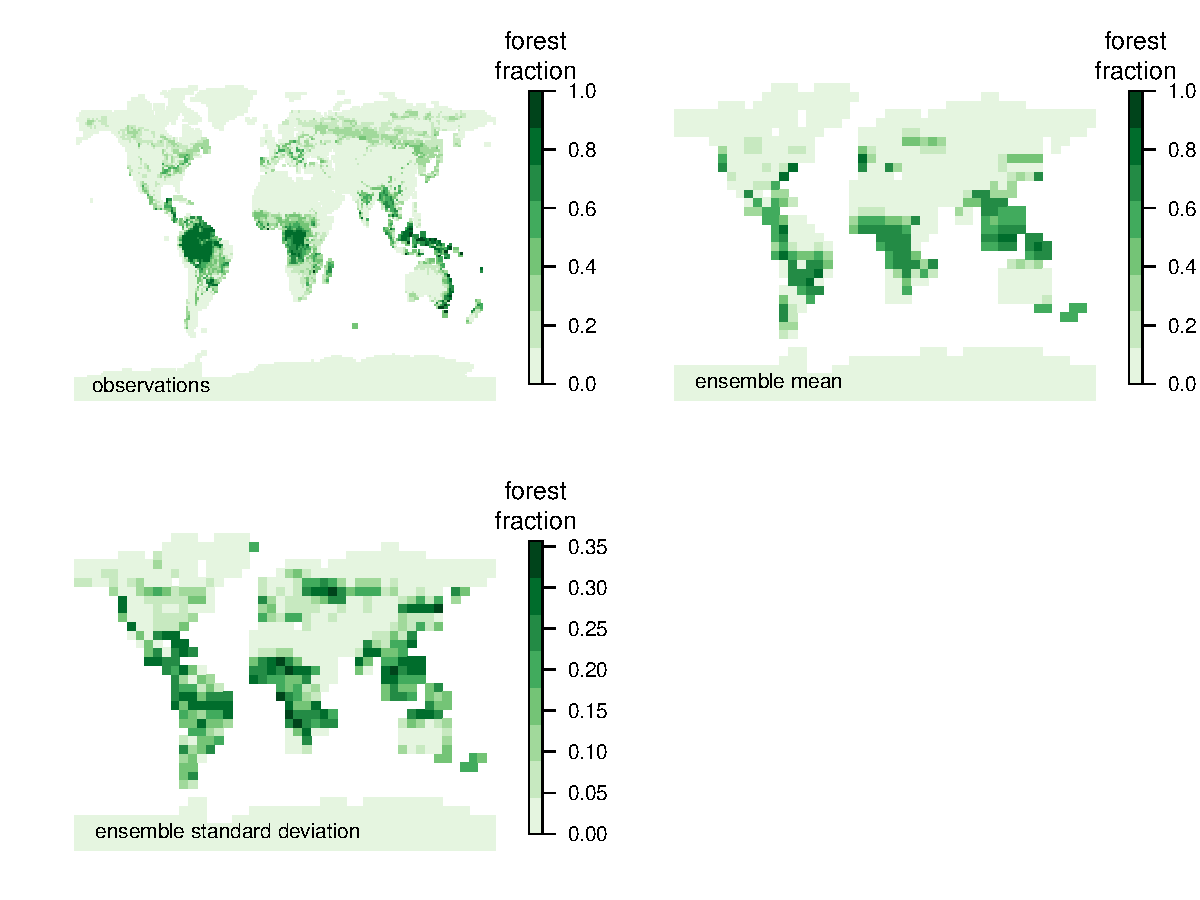
\includegraphics[width=12cm]{graphics/BL_obs_ensemble_mean_sd.pdf}
\caption{TEXT}
\label{fig:BL_obs_ensemble_mean_sd}
\end{figure}

\begin{figure}[t]
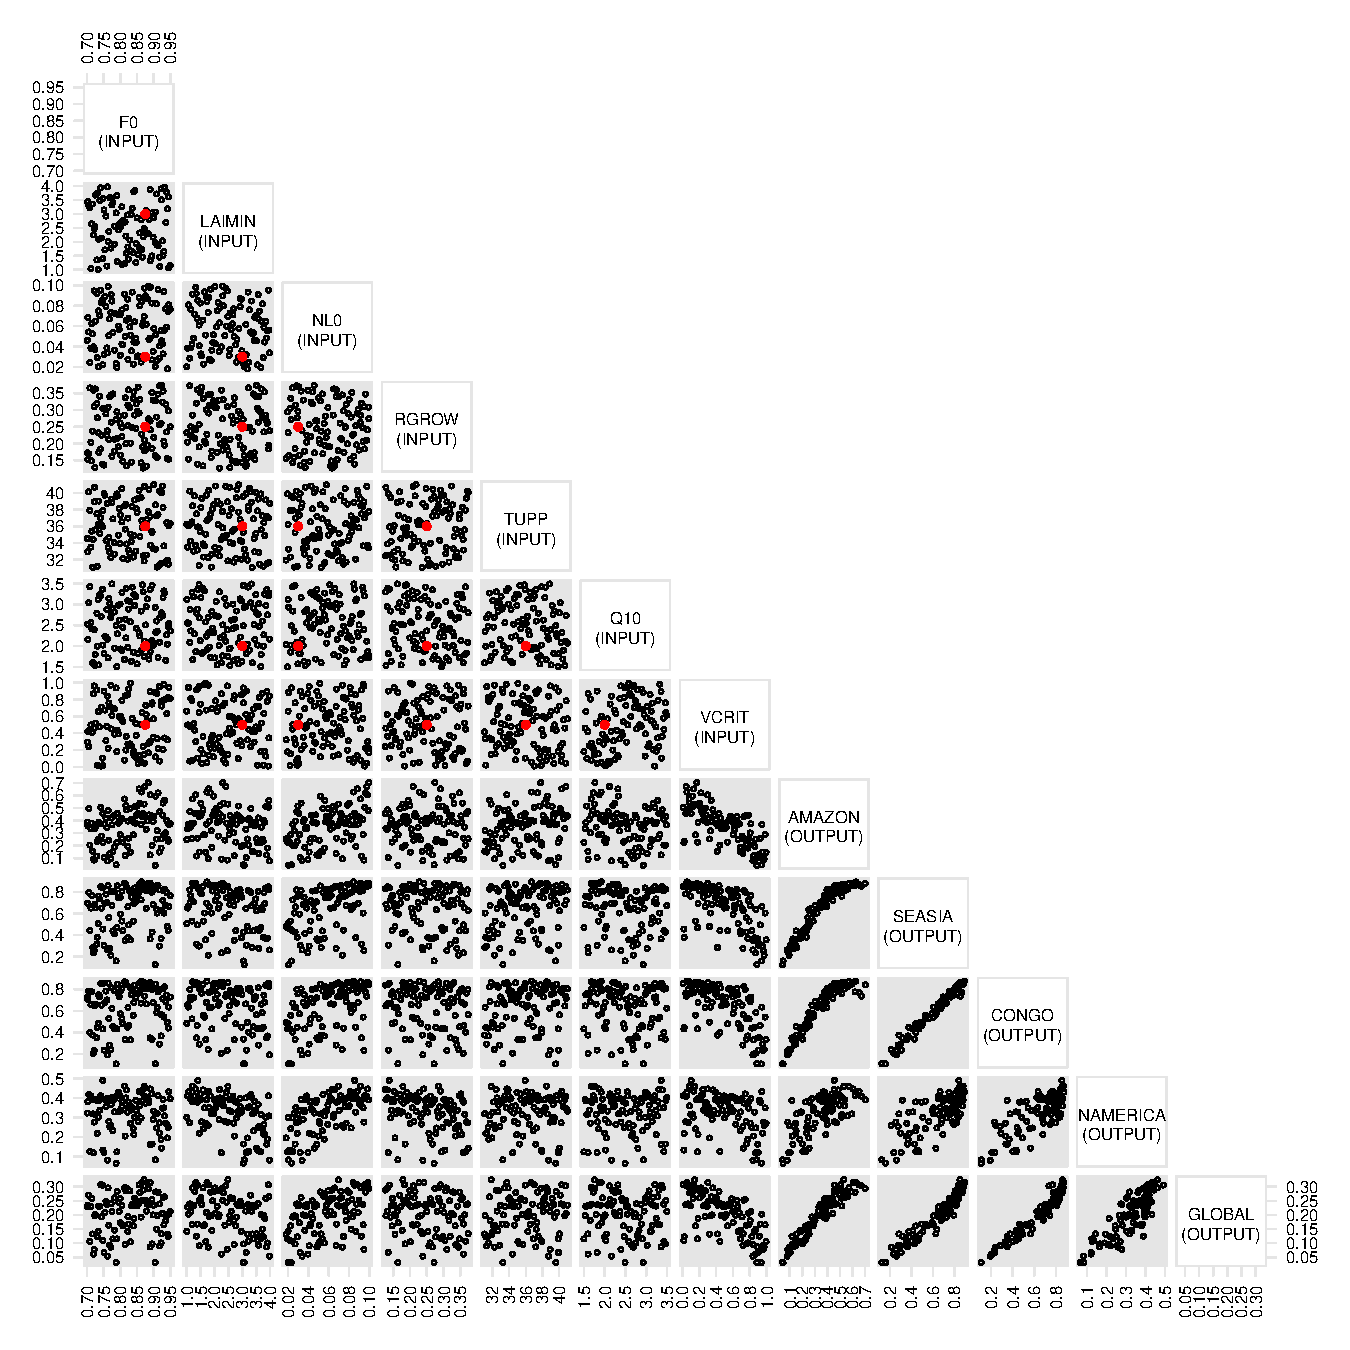
\includegraphics[width=12cm]{graphics/frac_pairs.pdf}
\caption{TEXT}
\label{fig:frac_pairs}
\end{figure}

\begin{figure}[t]
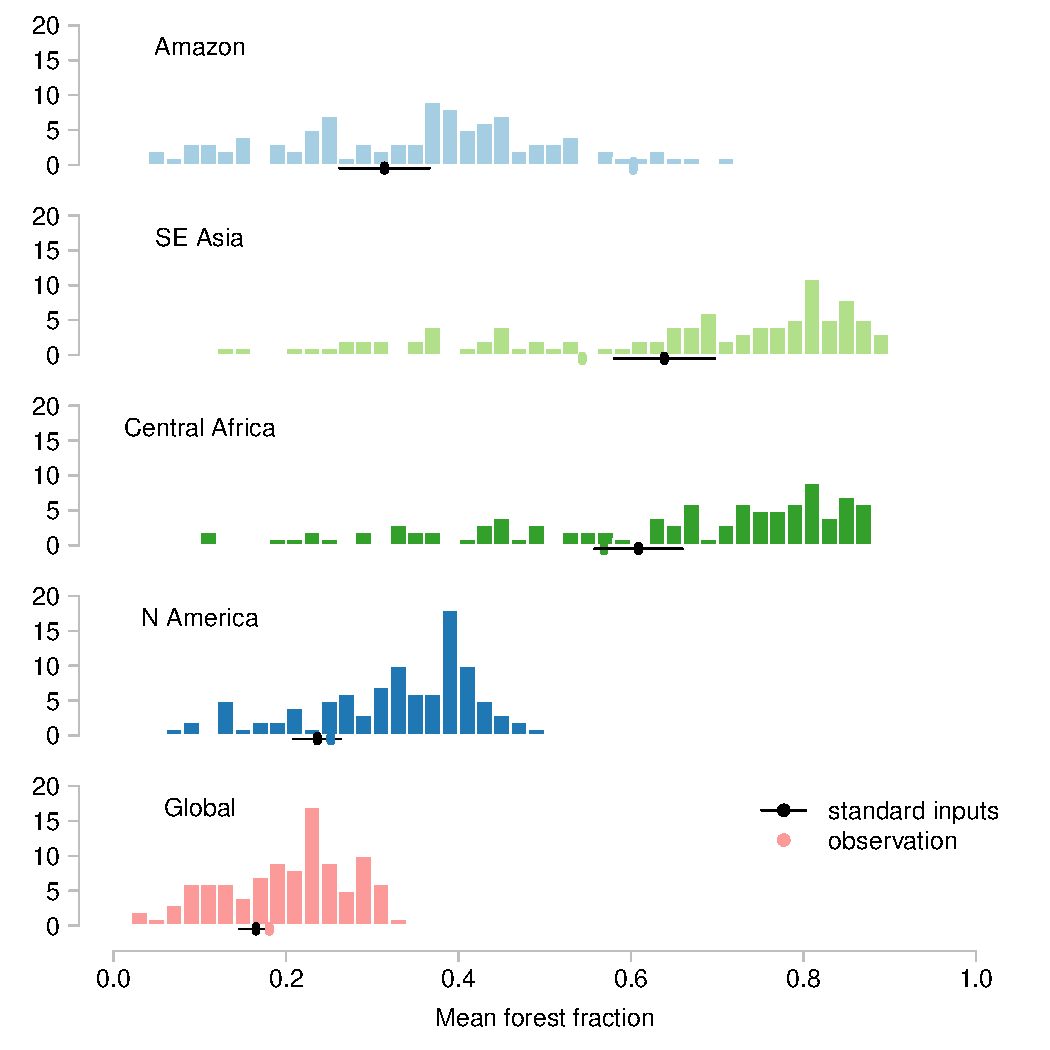
\includegraphics[width=12cm]{graphics/fraction_histogram_with_discrepancy_standard.pdf}
\caption{TEXT}
\label{fig:fraction_histogram_with_discrepancy_standard}
\end{figure}

\begin{figure}[t]
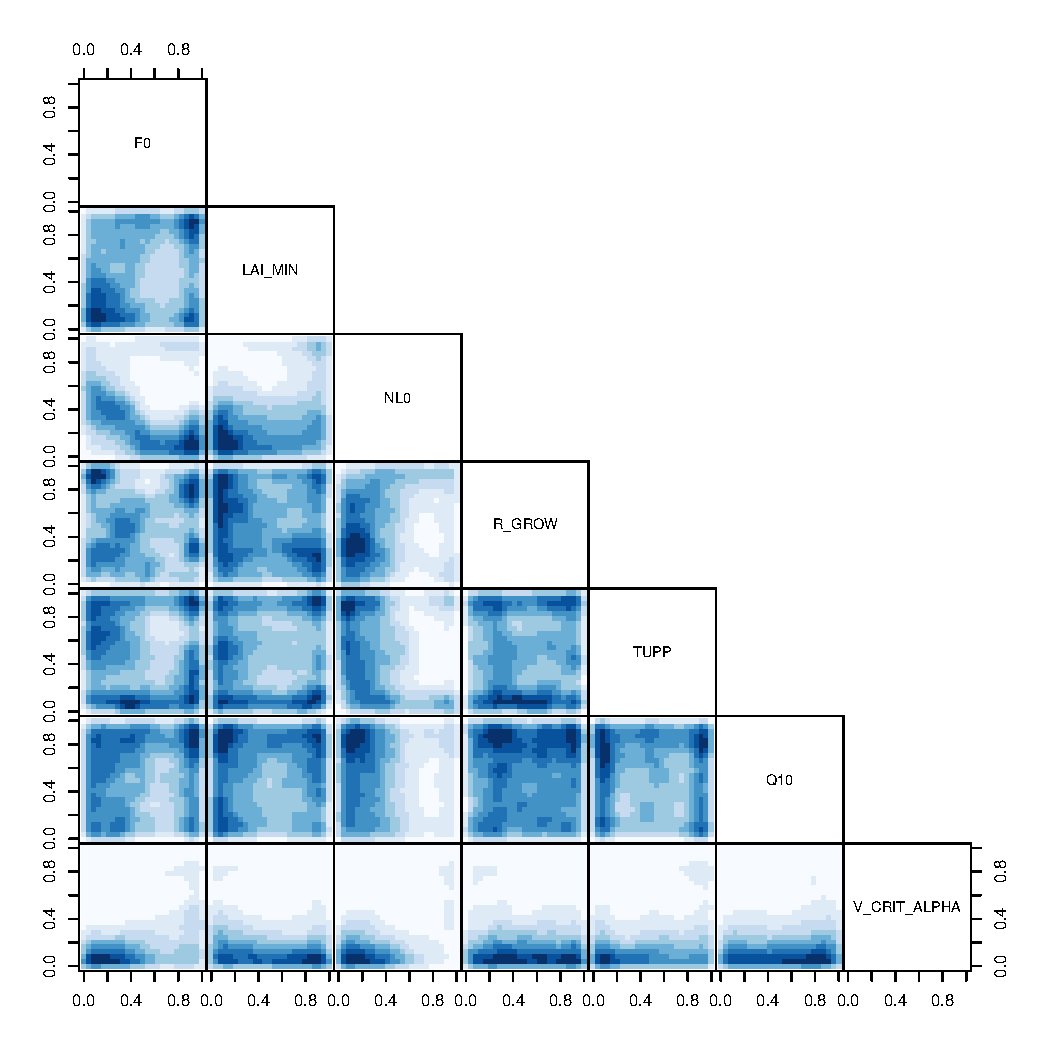
\includegraphics[width=12cm]{graphics/credible_NROY.pdf}
\caption{TEXT}
\label{fig:credible_NROY}
\end{figure}

\begin{figure}[t]
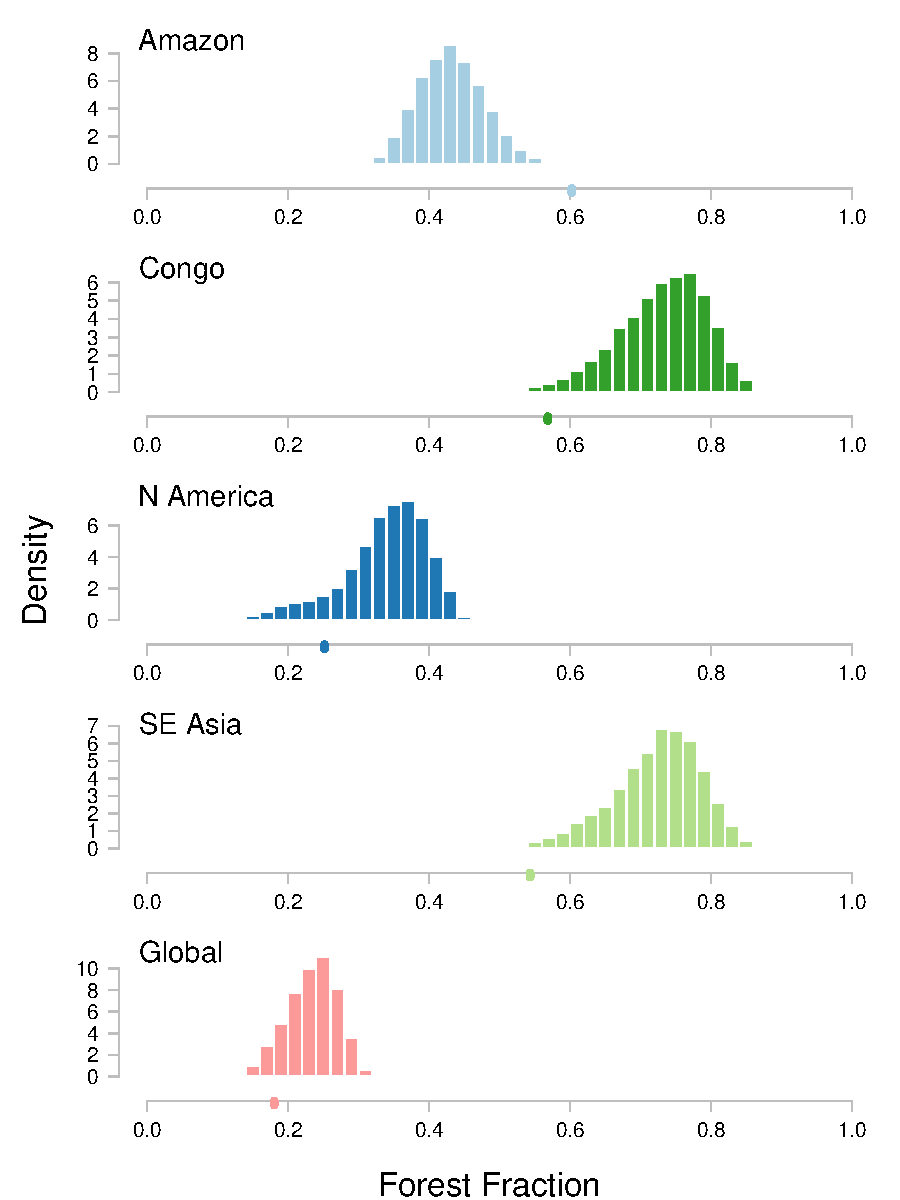
\includegraphics[width=12cm]{graphics/credible_NROY_hists.pdf}
\caption{TEXT}
\label{fig:credible_NROY_hists}
\end{figure}

\begin{figure}[t]
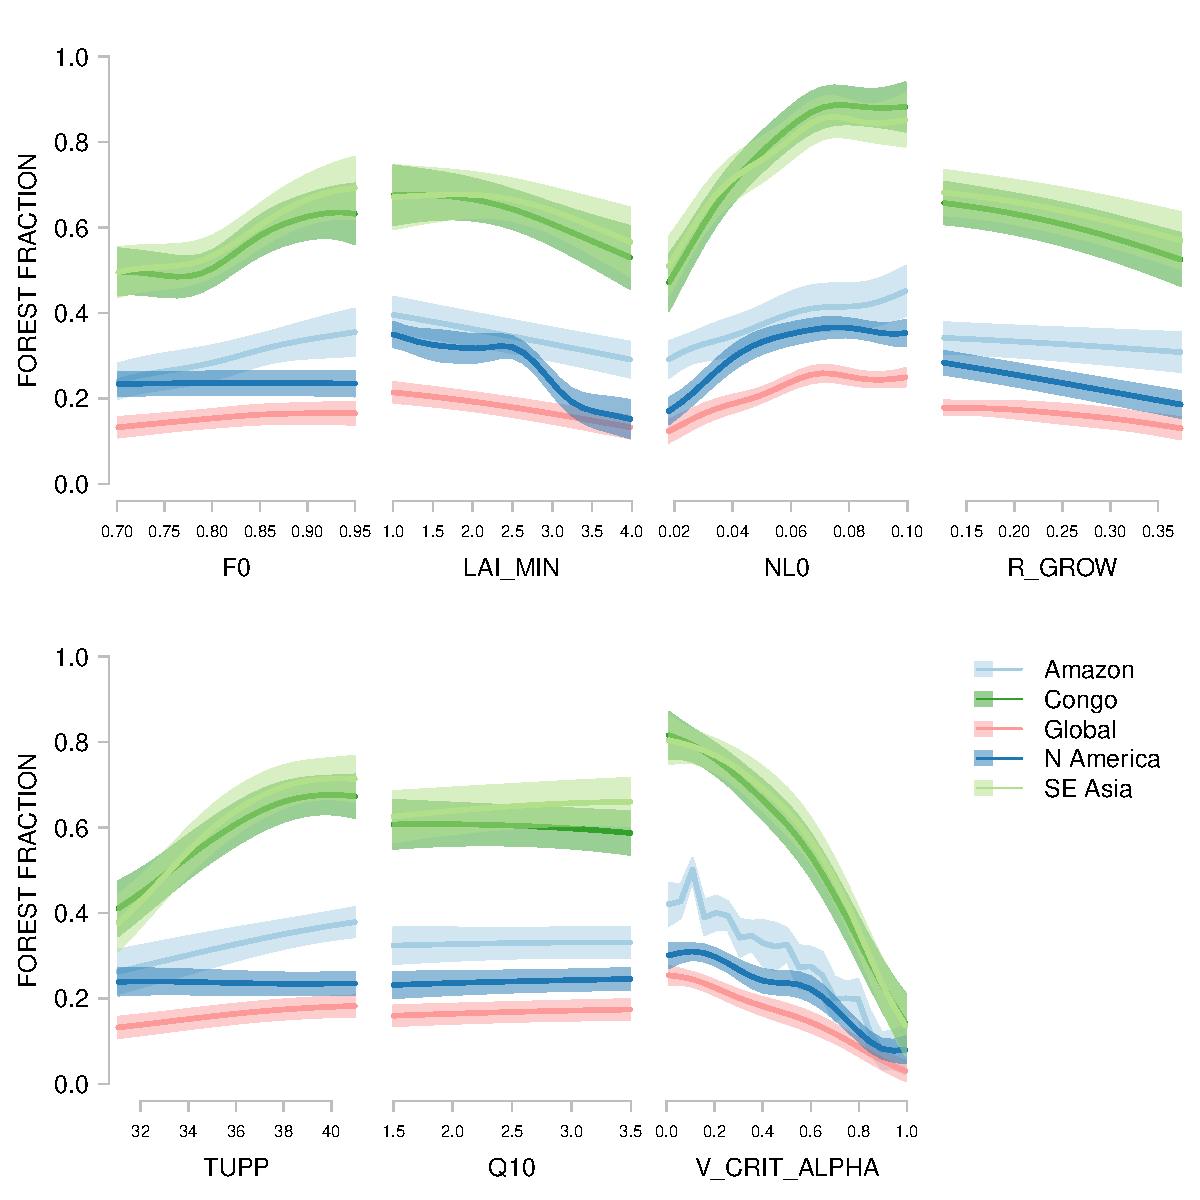
\includegraphics[width=12cm]{graphics/amaz_oat_sens.pdf}
\caption{TEXT}
\label{fig:amaz_oat_sens}
\end{figure}

\begin{figure}[t]
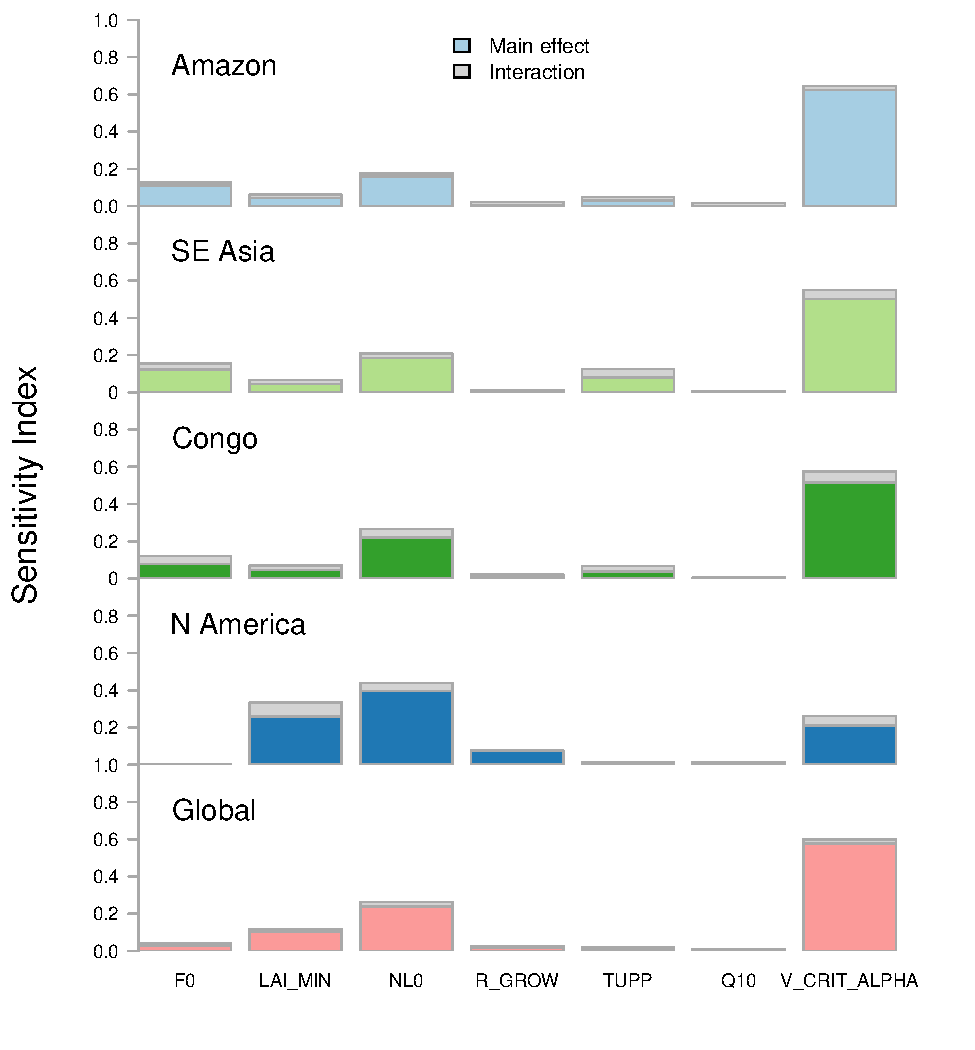
\includegraphics[width=12cm]{graphics/FAST_histograms.pdf}
\caption{TEXT}
\label{fig:FAST_histograms}
\end{figure}

\begin{figure}[t]
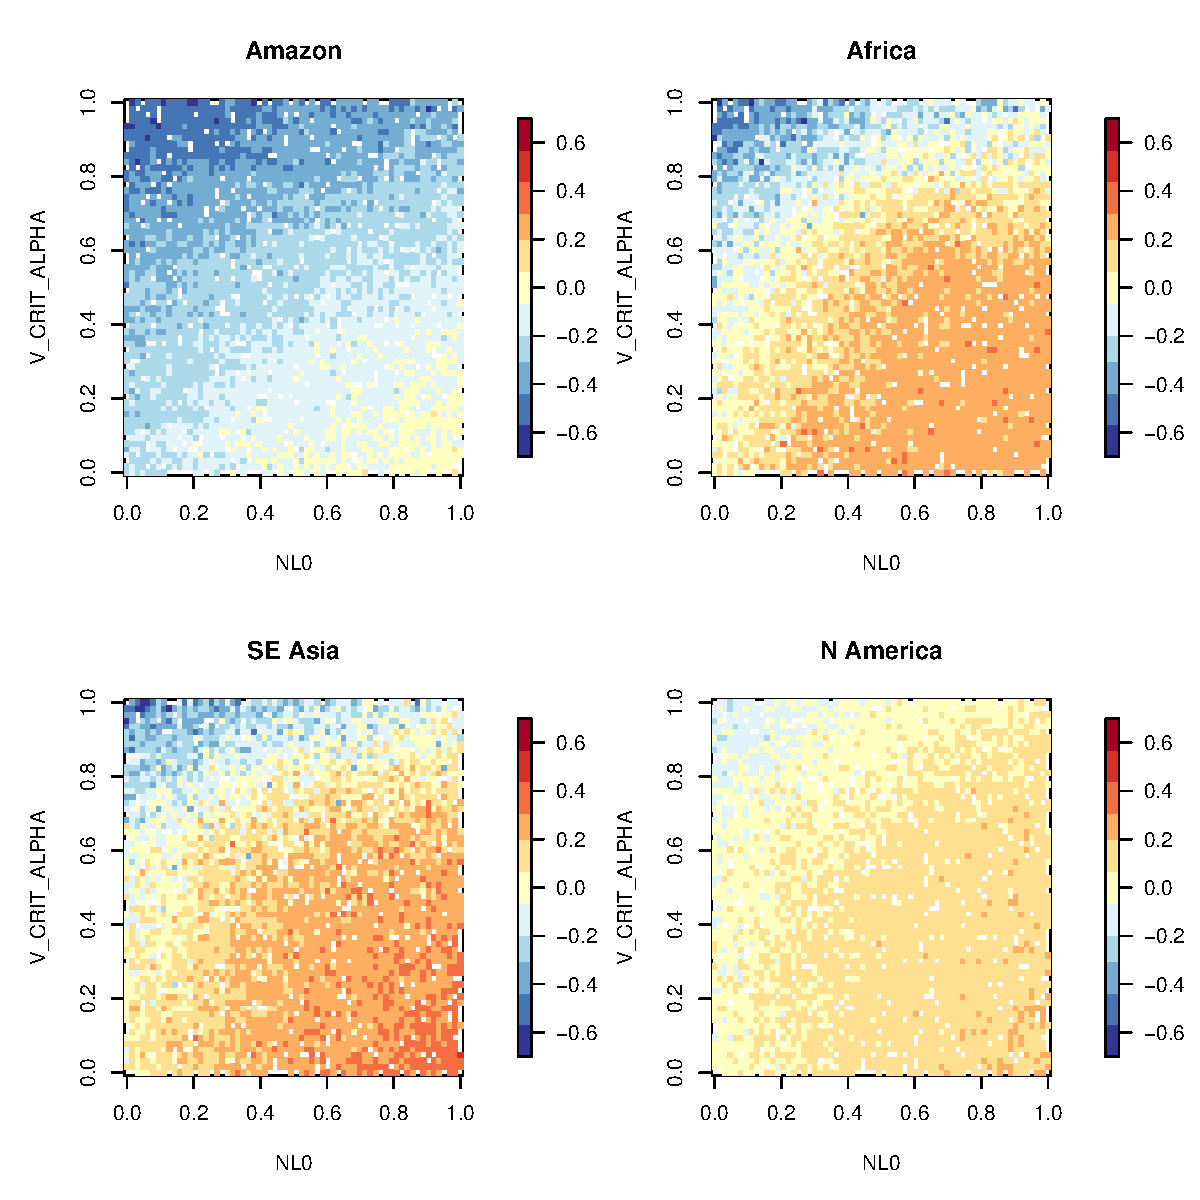
\includegraphics[width=12cm]{graphics/discrepancy_parameter_space.pdf}
\caption{TEXT}
\label{fig:discrepancy_parameter_space}
\end{figure}

\begin{figure}[t]
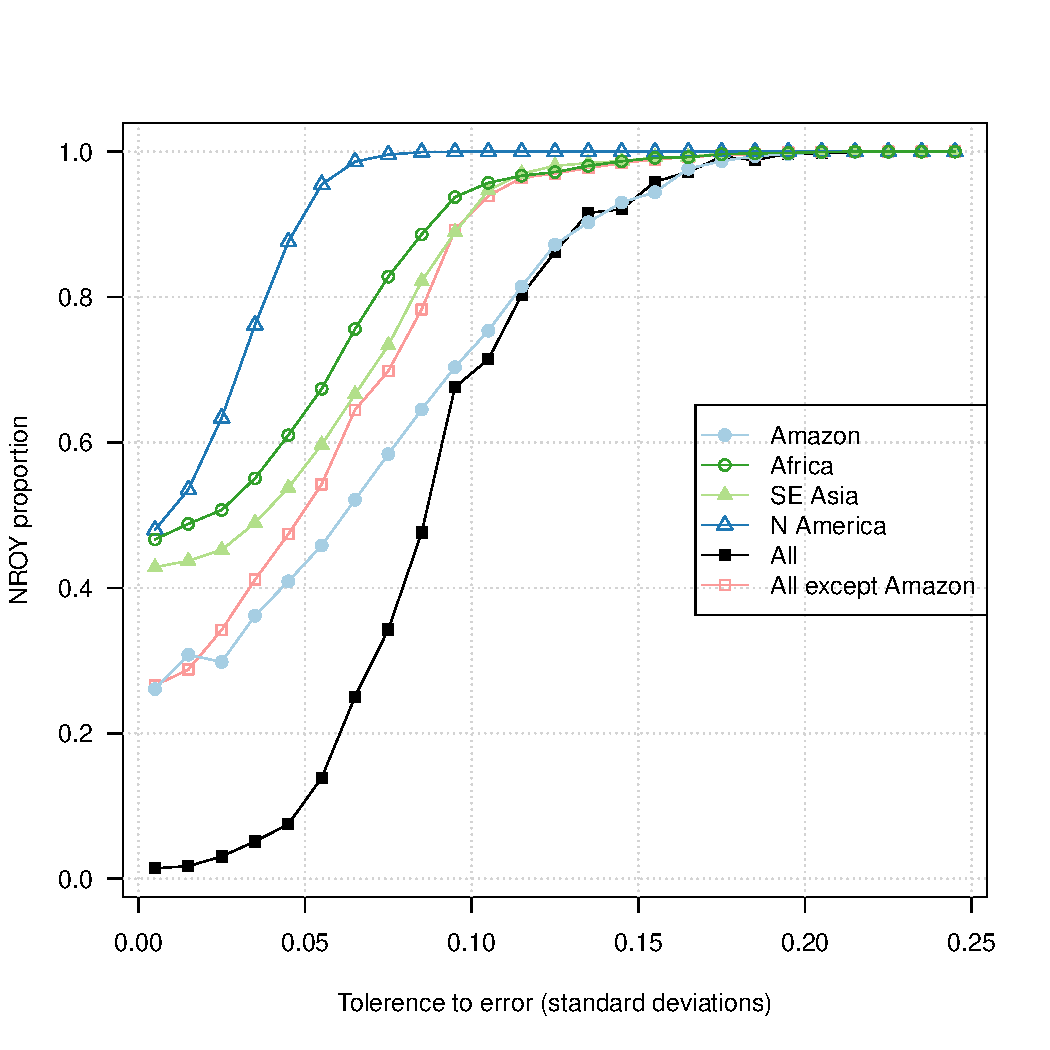
\includegraphics[width=12cm]{graphics/Prop_NROY_tolerance_unc.pdf}
\caption{TEXT}
\label{fig:Prop_NROY_tolerance_unc}
\end{figure}

\begin{figure}[t]
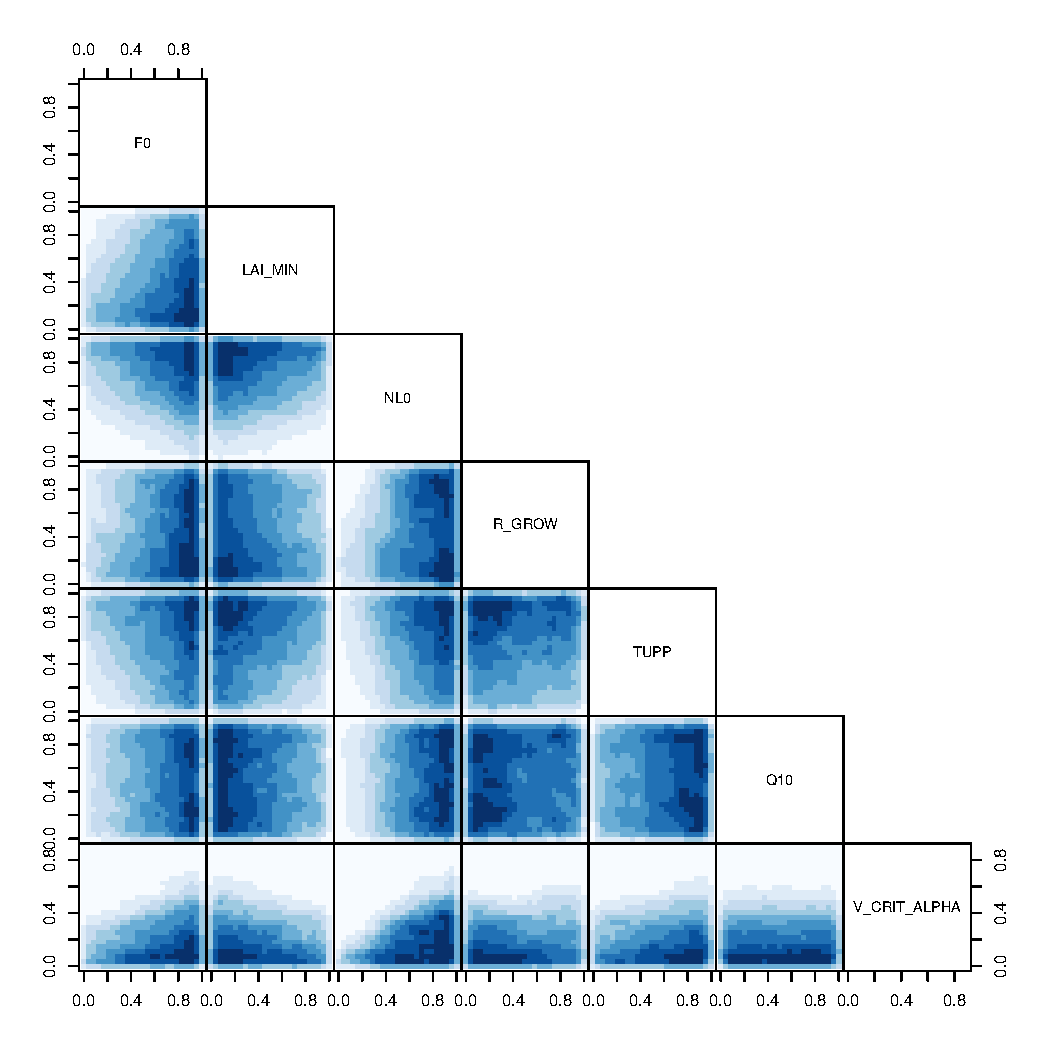
\includegraphics[width=12cm]{graphics/best_inputs_amazon.pdf}
\caption{TEXT}
\label{fig:best_inputs_amazon}
\end{figure}

\begin{figure}[t]
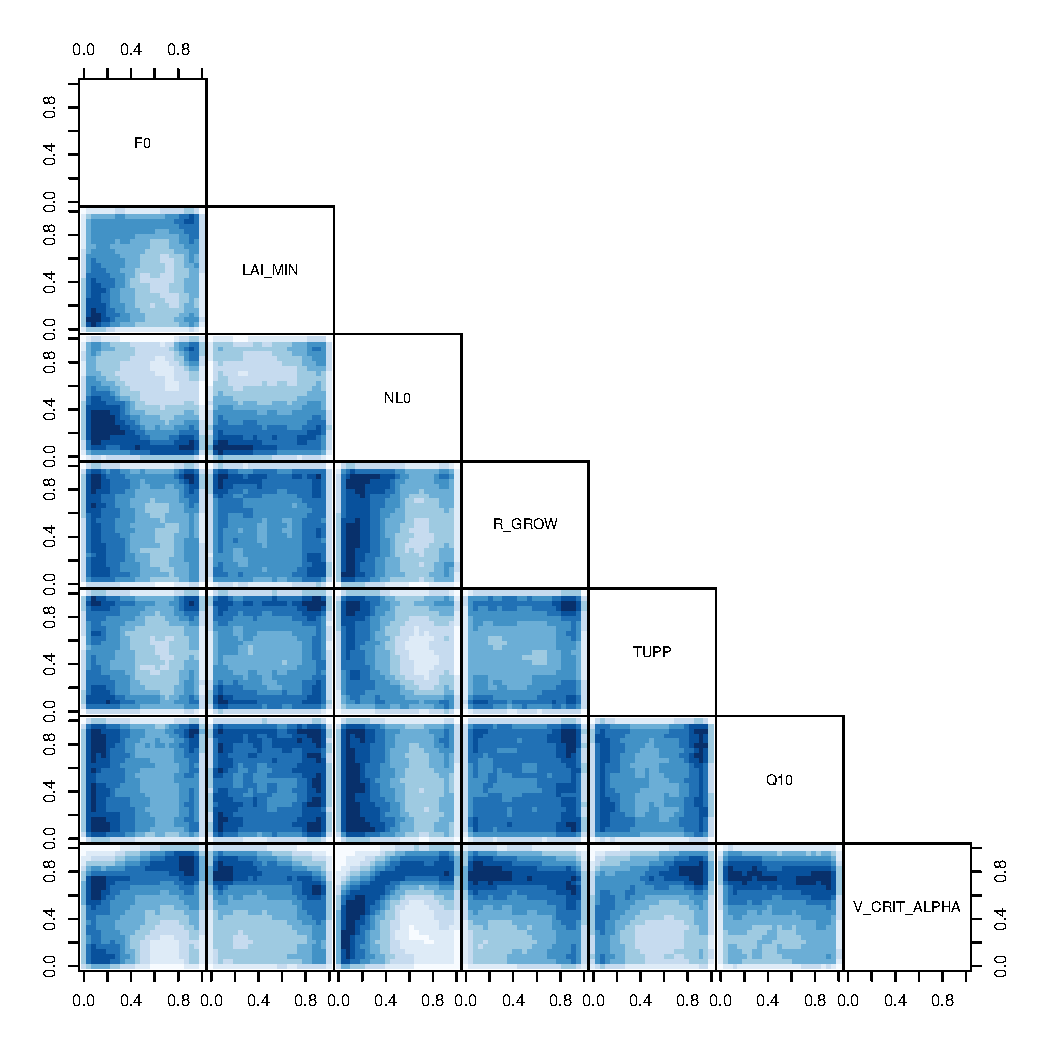
\includegraphics[width=12cm]{graphics/best_inputs_congo.pdf}
\caption{TEXT}
\label{fig:}
\end{figure}

\begin{figure}[t]
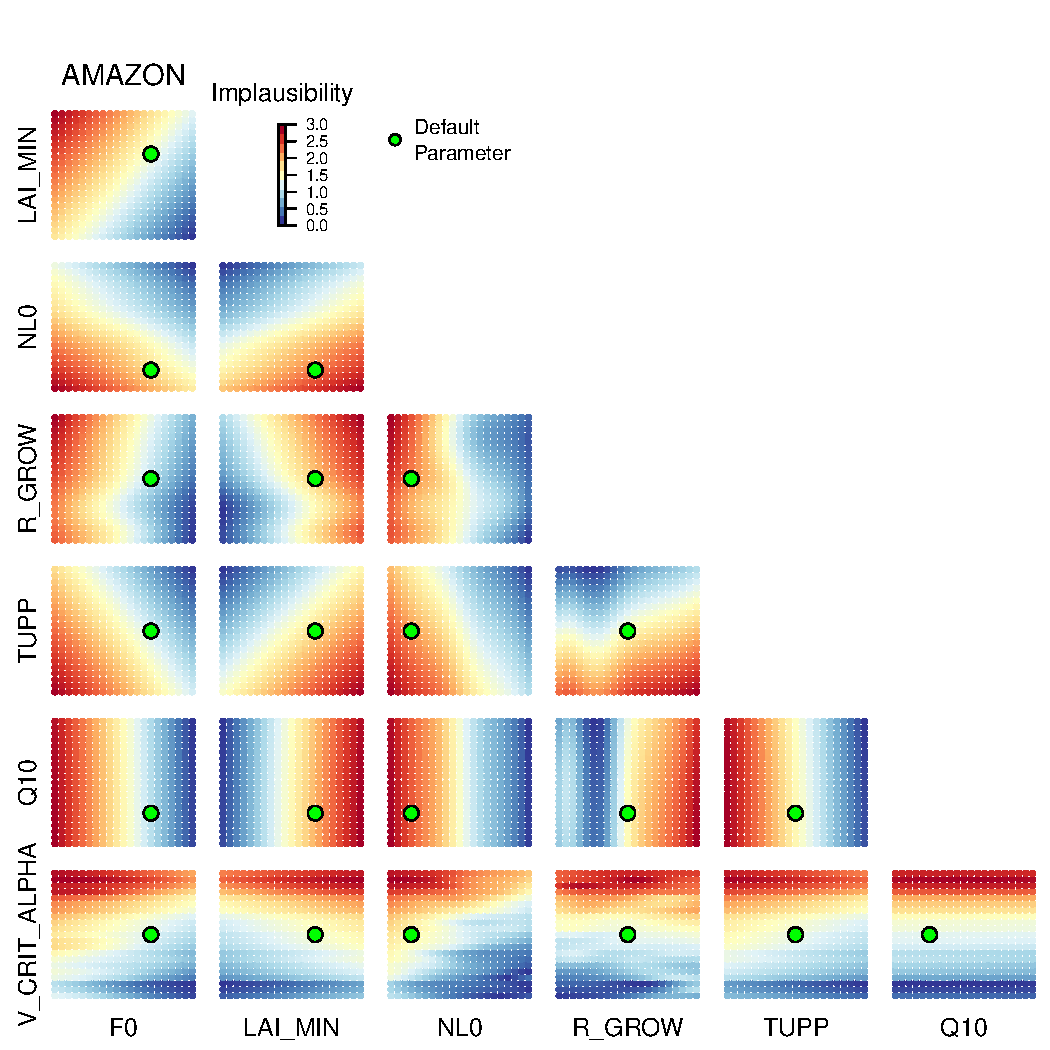
\includegraphics[width=12cm]{graphics/taat_amaz.pdf}
\caption{TEXT}
\label{fig:taat_amaz}
\end{figure}

\begin{figure}[t]
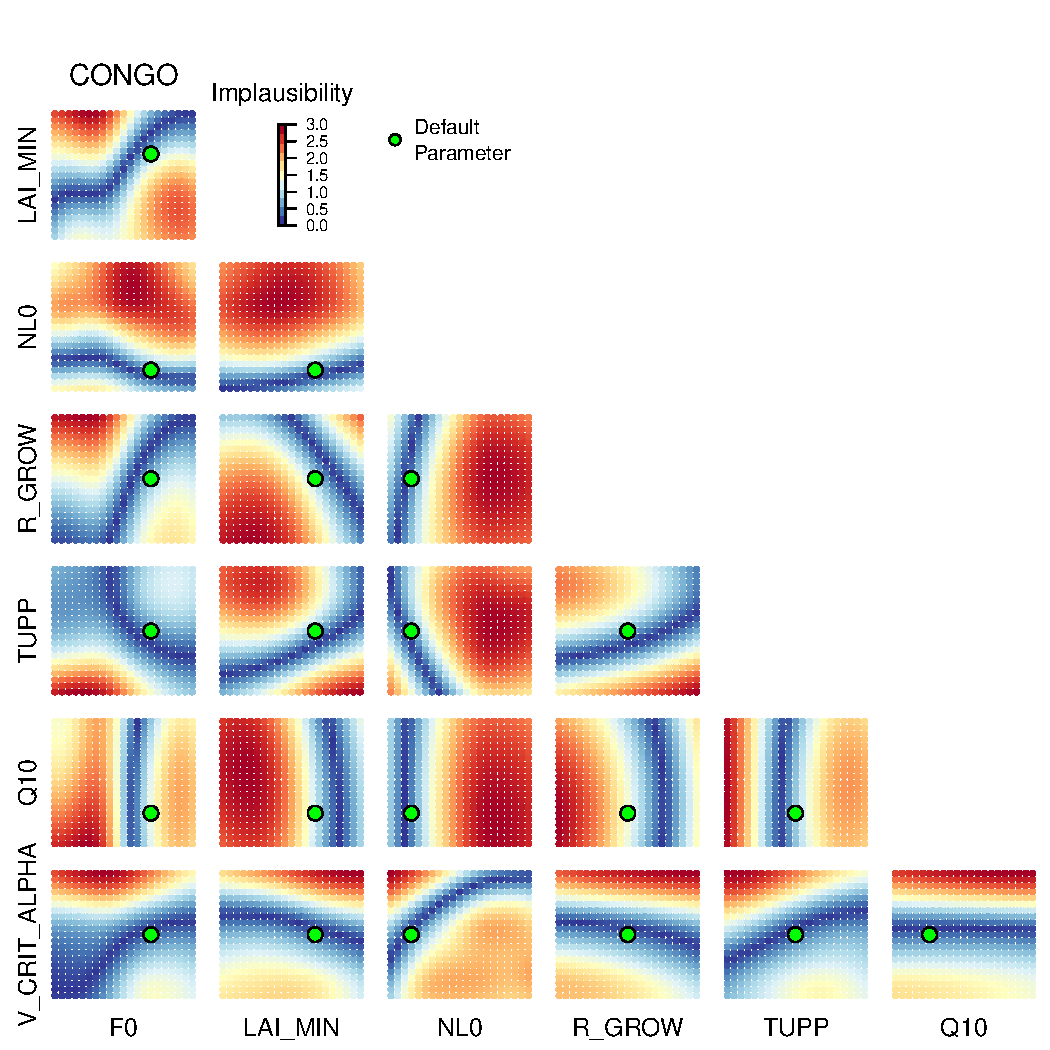
\includegraphics[width=12cm]{graphics/taat_congo.pdf}
\caption{TEXT}
\label{fig:}
\end{figure}

\begin{figure}[t]
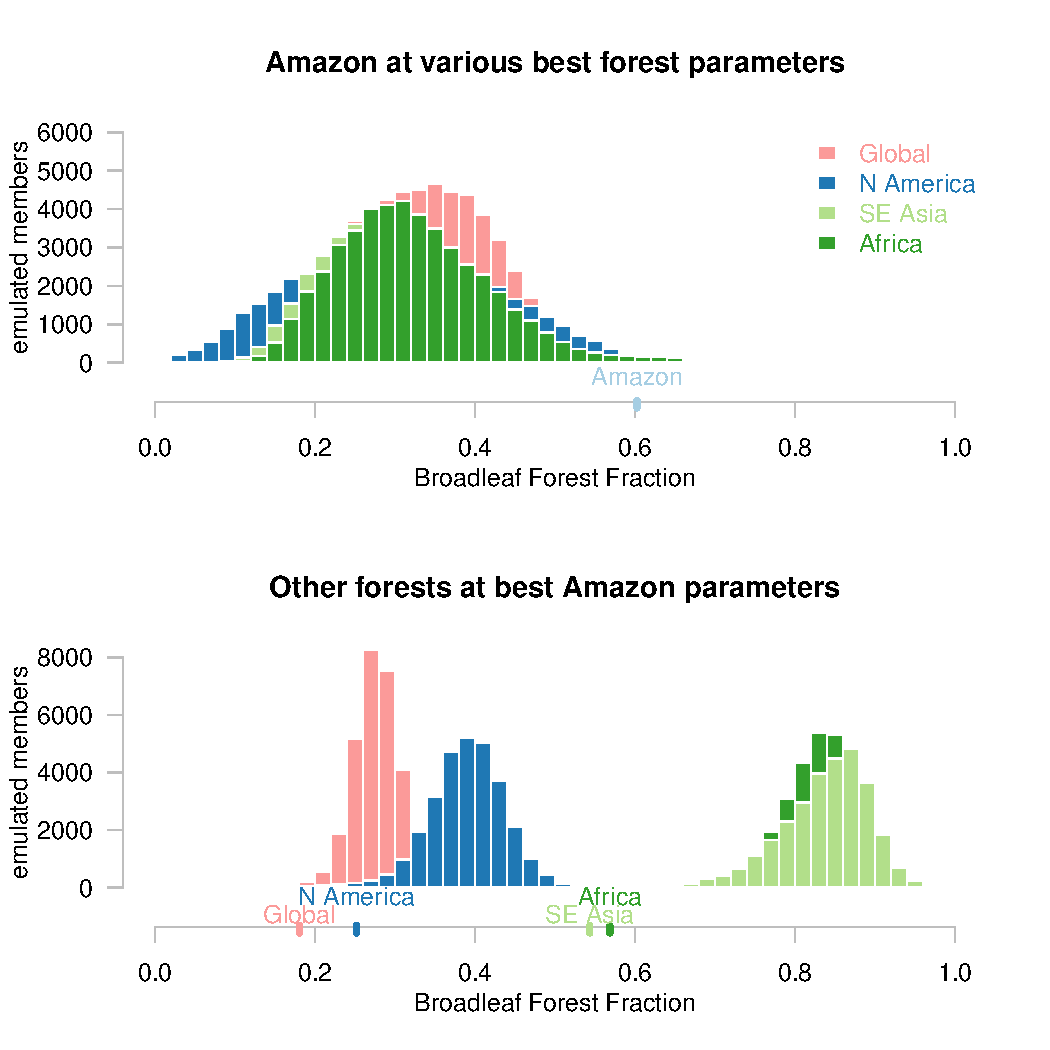
\includegraphics[width=12cm]{graphics/best_inputs_swaps_hists_Paired.pdf}
\caption{TEXT}
\label{fig:best_inputs_swaps_hists_Paired}
\end{figure}

\begin{figure}[t]
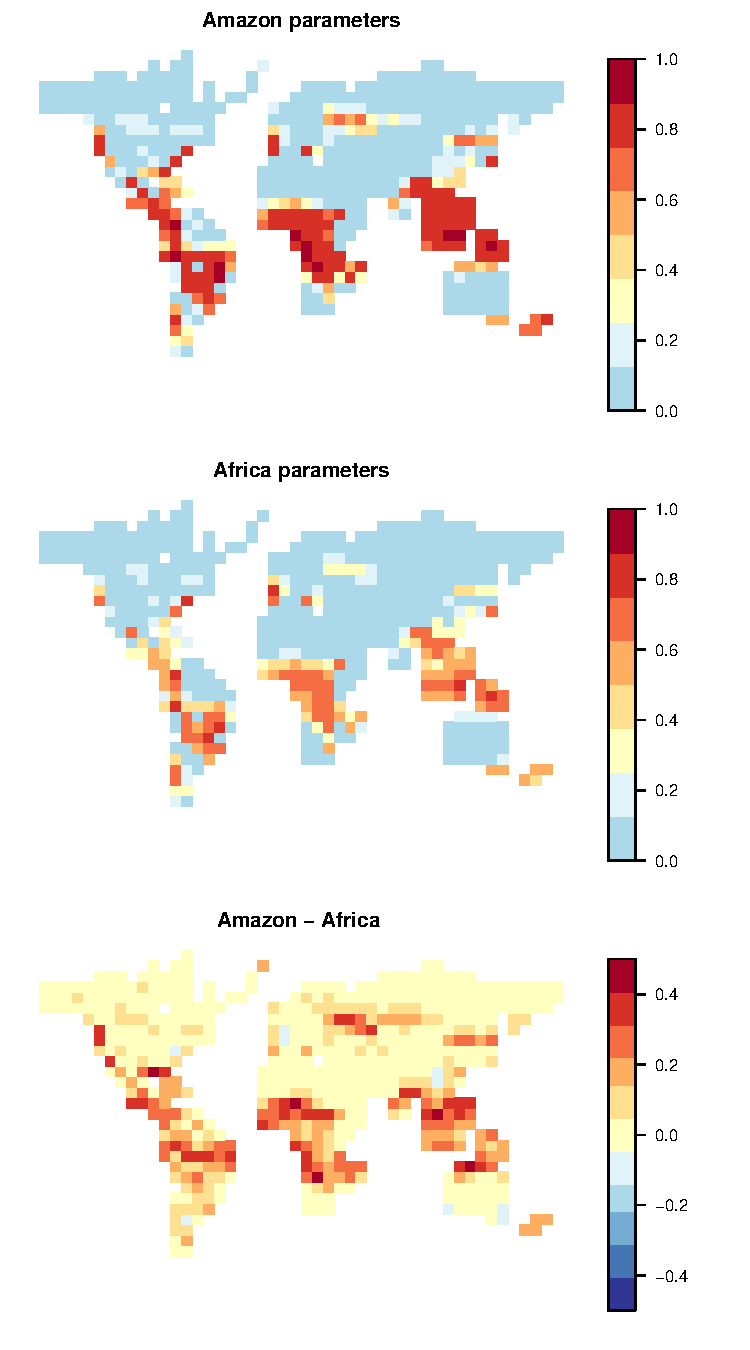
\includegraphics[width=8.3cm]{graphics/best_X_maps.pdf}
\caption{TEXT}
\label{fig:best_X_maps}
\end{figure}

\begin{figure}[t]
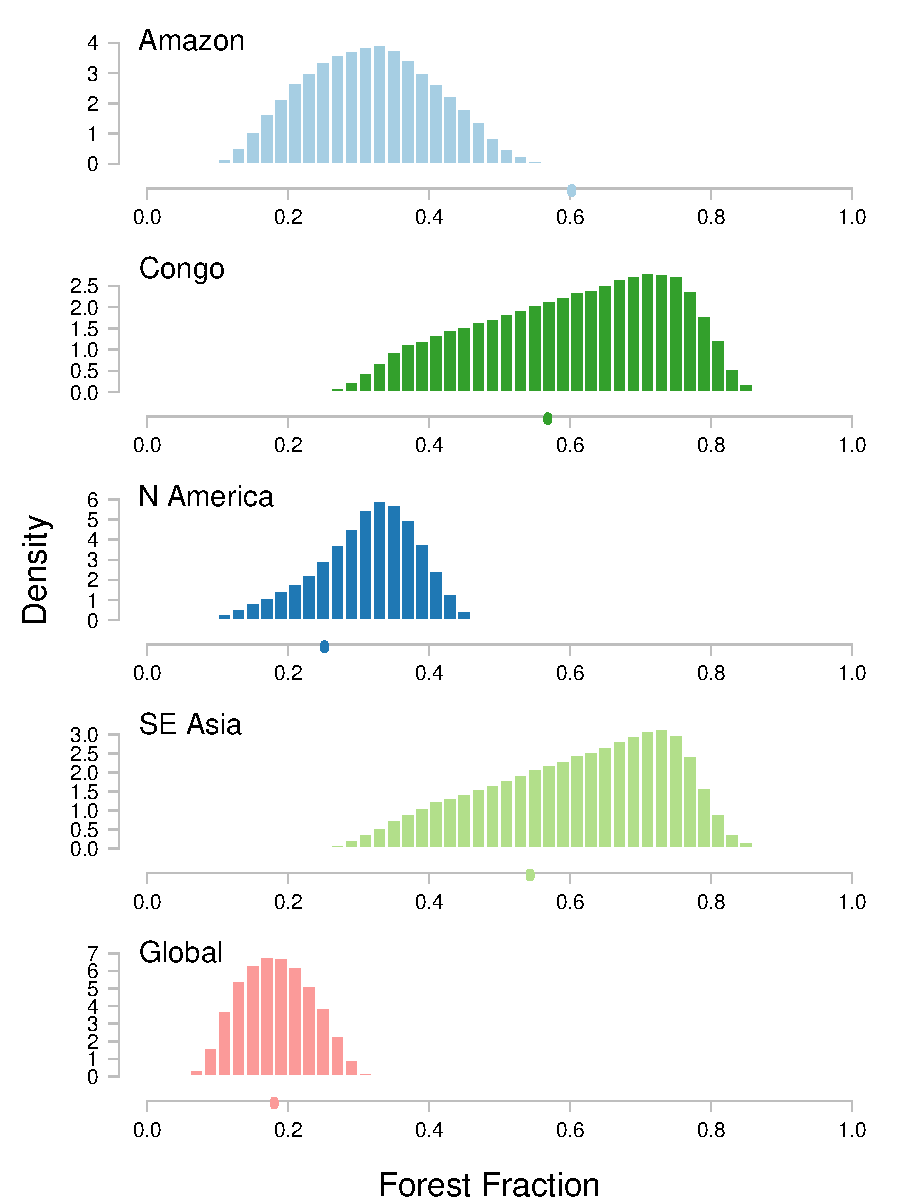
\includegraphics[width=12cm]{graphics/credible_NROY_hists_disc.pdf}
\caption{TEXT}
\label{fig:credible_NROY_hists_disc}
\end{figure}

\begin{figure}[t]
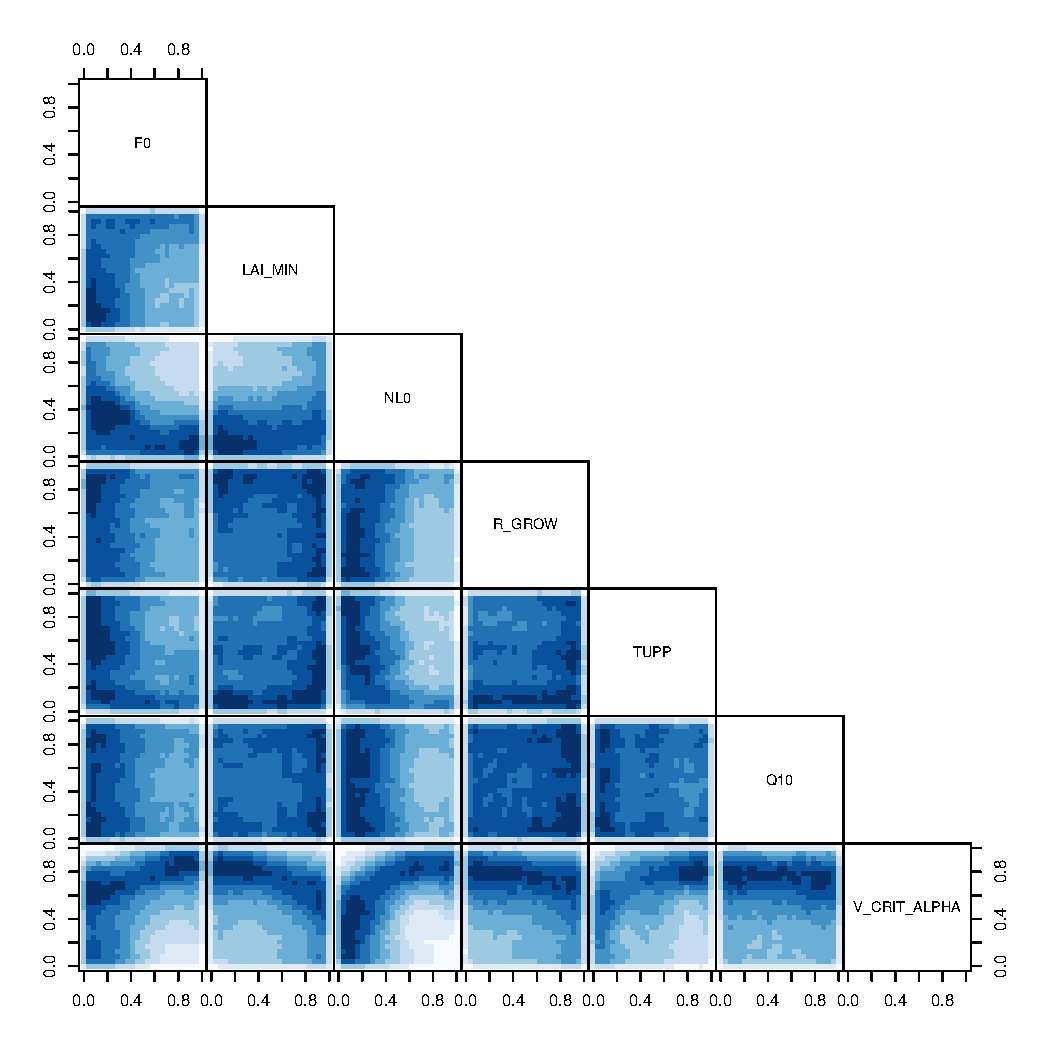
\includegraphics[width=12cm]{graphics/plausible_disc_input_space.pdf}
\caption{TEXT}
\label{fig:plausible_disc_input_space}
\end{figure}

\begin{figure}[t]
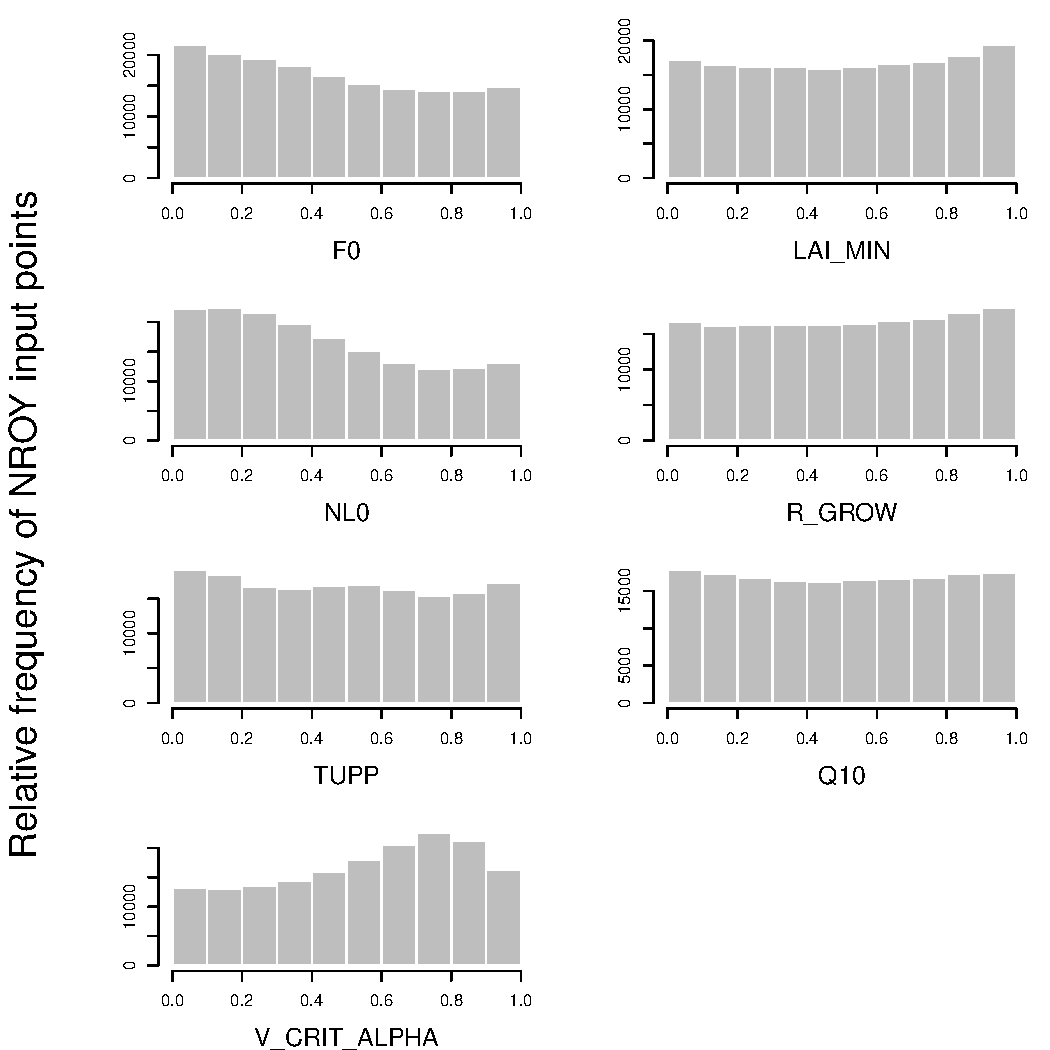
\includegraphics[width=12cm]{graphics/input_frequency_marginal.pdf}
\caption{TEXT}
\label{fig:input_frequency_marginal}
\end{figure}

%\begin{figure}[t]
%\includegraphics[width=12cm]{graphics/.pdf}
%\caption{TEXT}
%\label{fig:}
%\end{figure}



%% ONE-COLUMN FIGURES

%%f
%\begin{figure}[t]
%\includegraphics[width=8.3cm]{FILE NAME}
%\caption{TEXT}
%\end{figure}
%
%%% TWO-COLUMN FIGURES
%
%%f
%\begin{figure*}[t]
%\includegraphics[width=12cm]{FILE NAME}
%\caption{TEXT}
%\end{figure*}
%
%
%%% TABLES
%%%
%%% The different columns must be seperated with a & command and should
%%% end with \\ to identify the column brake.
%
%%% ONE-COLUMN TABLE
%
%%t
%\begin{table}[t]
%\caption{TEXT}
%\begin{tabular}{column = lcr}
%\tophline
%
%\middlehline
%
%\bottomhline
%\end{tabular}
%\belowtable{} % Table Footnotes
%\end{table}
%
%%% TWO-COLUMN TABLE
%
%%t
%\begin{table*}[t]
%\caption{TEXT}
%\begin{tabular}{column = lcr}
%\tophline
%
%\middlehline
%
%\bottomhline
%\end{tabular}
%\belowtable{} % Table Footnotes
%\end{table*}
%
%
%%% NUMBERING OF FIGURES AND TABLES
%%%
%%% If figures and tables must be numbered 1a, 1b, etc. the following command
%%% should be inserted before the begin{} command.
%
%\addtocounter{figure}{-1}\renewcommand{\thefigure}{\arabic{figure}a}
%
%
%%% MATHEMATICAL EXPRESSIONS
%
%%% All papers typeset by Copernicus Publications follow the math typesetting regulations
%%% given by the IUPAC Green Book (IUPAC: Quantities, Units and Symbols in Physical Chemistry,
%%% 2nd Edn., Blackwell Science, available at: http://old.iupac.org/publications/books/gbook/green_book_2ed.pdf, 1993).
%%%
%%% Physical quantities/variables are typeset in italic font (t for time, T for Temperature)
%%% Indices which are not defined are typeset in italic font (x, y, z, a, b, c)
%%% Items/objects which are defined are typeset in roman font (Car A, Car B)
%%% Descriptions/specifications which are defined by itself are typeset in roman font (abs, rel, ref, tot, net, ice)
%%% Abbreviations from 2 letters are typeset in roman font (RH, LAI)
%%% Vectors are identified in bold italic font using \vec{x}
%%% Matrices are identified in bold roman font
%%% Multiplication signs are typeset using the LaTeX commands \times (for vector products, grids, and exponential notations) or \cdot
%%% The character * should not be applied as mutliplication sign
%
%
%%% EQUATIONS
%
%%% Single-row equation
%
%\begin{equation}
%
%\end{equation}
%
%%% Multiline equation
%
%\begin{align}
%& 3 + 5 = 8\\
%& 3 + 5 = 8\\
%& 3 + 5 = 8
%\end{align}
%
%
%%% MATRICES
%
%\begin{matrix}
%x & y & z\\
%x & y & z\\
%x & y & z\\
%\end{matrix}
%
%
%%% ALGORITHM
%
%\begin{algorithm}
%\caption{�}
%\label{a1}
%\begin{algorithmic}
%�
%\end{algorithmic}
%\end{algorithm}
%
%
%%% CHEMICAL FORMULAS AND REACTIONS
%
%%% For formulas embedded in the text, please use \chem{}
%
%%% The reaction environment creates labels including the letter R, i.e. (R1), (R2), etc.
%
%\begin{reaction}
%%% \rightarrow should be used for normal (one-way) chemical reactions
%%% \rightleftharpoons should be used for equilibria
%%% \leftrightarrow should be used for resonance structures
%\end{reaction}
%
%
%%% PHYSICAL UNITS
%%%
%%% Please use \unit{} and apply the exponential notation


\end{document}
